% ICAART 2027 — revisão de 2026-09-13.
% Compilar com o template SCITEPRESS (SCITEPRESS.sty + apalike.bst), p.ex. no Overleaf.
% Números: todos vêm de tables/macros.tex e tables/*.tex, gerados por
%   python study/analysis/form_agreement.py
% Não digitar número à mão. Pendências do autor aparecem em vermelho (\TODO).

\documentclass[a4paper,twoside]{article}

\usepackage{epsfig}
\usepackage{subcaption}
\usepackage{calc}
\usepackage{amssymb}
\usepackage{amstext}
\usepackage{amsmath}
\usepackage{amsthm}
\usepackage{multicol}
\usepackage{pslatex}
\usepackage{apalike}
\usepackage{booktabs}
\usepackage{tabularx}
\usepackage{adjustbox}
\usepackage{url}
\usepackage{xcolor}
\usepackage{tikz}
\usetikzlibrary{arrows.meta,positioning,calc,shapes.geometric}
\usepackage{SCITEPRESS} % other packages must be loaded BEFORE SCITEPRESS.sty

% Reserva: o SCITEPRESS.sty oficial define estes comandos. Se o projeto não
% estiver usando o .sty do template, isto evita "Undefined control sequence"
% no bloco de autores. Com o .sty certo, \providecommand não faz nada.
\providecommand{\authorname}[1]{#1\\}
\providecommand{\affiliation}[1]{\textit{#1}\\}
\providecommand{\email}[1]{\textit{#1}}
\providecommand{\sup}[1]{$^{#1}$}
\providecommand{\orcidAuthor}[1]{}

\newcommand{\TODO}[1]{\textcolor{red}{[TODO: #1]}}
% --- início de tables/macros.tex (gerado) ---
% GERADO por study/analysis/form_agreement.py — não editar à mão.
\newcommand{\NRaters}{18}
\newcommand{\NPosts}{10}
\newcommand{\NCHperDim}{180}
\newcommand{\NHHperDim}{1,530}
\newcommand{\HHexAll}{28.4\%}
\newcommand{\HHwAll}{68.7\%}
\newcommand{\CHexAll}{31.8\%}
\newcommand{\CHwAll}{78.6\%}
\newcommand{\CHchanceExAll}{31.9\%}
\newcommand{\CHchanceWAll}{78.4\%}
\newcommand{\ConstExAll}{39.2\%}
\newcommand{\ConstWAll}{86.5\%}
\newcommand{\CHexLo}{22.8\%}
\newcommand{\CHexHi}{40.8\%}
\newcommand{\CHwLo}{66.9\%}
\newcommand{\CHwHi}{88.2\%}
\newcommand{\HHexLo}{21.0\%}
\newcommand{\HHexHi}{36.5\%}
\newcommand{\HHwLo}{55.2\%}
\newcommand{\HHwHi}{81.0\%}
\newcommand{\DiffExLo}{$-$6.9}
\newcommand{\DiffExHi}{+10.5}
\newcommand{\DiffWLo}{+0.0}
\newcommand{\DiffWHi}{+17.4}
\newcommand{\ChanceDiffExLo}{$-$3.2}
\newcommand{\ChanceDiffExHi}{+3.0}
\newcommand{\ChanceDiffWLo}{$-$2.0}
\newcommand{\ChanceDiffWHi}{+2.6}
\newcommand{\HHchanceExAll}{28.8\%}
\newcommand{\HHchanceWAll}{69.0\%}
\newcommand{\HHChanceDiffExLo}{$-$5.5}
\newcommand{\HHChanceDiffExHi}{+1.3}
\newcommand{\HHChanceDiffWLo}{$-$3.7}
\newcommand{\HHChanceDiffWHi}{+1.2}
\newcommand{\HumMeanCla}{3.91}
\newcommand{\CriMeanCla}{4.00}
\newcommand{\BiasCla}{+0.09}
\newcommand{\BiasLoCla}{$-$0.26}
\newcommand{\BiasHiCla}{+0.48}
\newcommand{\MAECla}{0.76}
\newcommand{\KappaCla}{0.00}
\newcommand{\RhoCla}{n/a}
\newcommand{\AlphaCla}{$-$0.02}
\newcommand{\AlphaLoCla}{$-$0.05}
\newcommand{\AlphaHiCla}{$-$0.01}
\newcommand{\CHexCla}{41.1\%}
\newcommand{\HHexCla}{31.7\%}
\newcommand{\CriDistinctCla}{1}
\newcommand{\PostMeanSDCla}{0.21}
\newcommand{\HumModeCla}{4}
\newcommand{\VarPostCla}{3\%}
\newcommand{\VarRaterCla}{43\%}
\newcommand{\HumMeanRel}{3.74}
\newcommand{\CriMeanRel}{3.20}
\newcommand{\BiasRel}{$-$0.54}
\newcommand{\BiasLoRel}{$-$0.98}
\newcommand{\BiasHiRel}{$-$0.05}
\newcommand{\MAERel}{1.12}
\newcommand{\KappaRel}{0.01}
\newcommand{\RhoRel}{0.13}
\newcommand{\AlphaRel}{$-$0.01}
\newcommand{\AlphaLoRel}{$-$0.05}
\newcommand{\AlphaHiRel}{0.02}
\newcommand{\CHexRel}{21.7\%}
\newcommand{\HHexRel}{26.9\%}
\newcommand{\CriDistinctRel}{2}
\newcommand{\PostMeanSDRel}{0.24}
\newcommand{\HumModeRel}{4}
\newcommand{\VarPostRel}{4\%}
\newcommand{\VarRaterRel}{42\%}
\newcommand{\HumMeanPro}{3.93}
\newcommand{\CriMeanPro}{4.10}
\newcommand{\BiasPro}{+0.17}
\newcommand{\BiasLoPro}{$-$0.22}
\newcommand{\BiasHiPro}{+0.56}
\newcommand{\MAEPro}{0.75}
\newcommand{\KappaPro}{0.05}
\newcommand{\RhoPro}{0.53}
\newcommand{\AlphaPro}{$-$0.01}
\newcommand{\AlphaLoPro}{$-$0.04}
\newcommand{\AlphaHiPro}{0.00}
\newcommand{\CHexPro}{42.2\%}
\newcommand{\HHexPro}{30.1\%}
\newcommand{\CriDistinctPro}{2}
\newcommand{\PostMeanSDPro}{0.22}
\newcommand{\HumModePro}{4}
\newcommand{\VarPostPro}{4\%}
\newcommand{\VarRaterPro}{44\%}
\newcommand{\HumMeanEng}{3.66}
\newcommand{\CriMeanEng}{3.30}
\newcommand{\BiasEng}{$-$0.36}
\newcommand{\BiasLoEng}{$-$0.84}
\newcommand{\BiasHiEng}{+0.13}
\newcommand{\MAEEng}{1.11}
\newcommand{\KappaEng}{0.00}
\newcommand{\RhoEng}{0.04}
\newcommand{\AlphaEng}{$-$0.02}
\newcommand{\AlphaLoEng}{$-$0.05}
\newcommand{\AlphaHiEng}{0.01}
\newcommand{\CHexEng}{22.2\%}
\newcommand{\HHexEng}{25.2\%}
\newcommand{\CriDistinctEng}{2}
\newcommand{\PostMeanSDEng}{0.21}
\newcommand{\HumModeEng}{4}
\newcommand{\VarPostEng}{3\%}
\newcommand{\VarRaterEng}{42\%}
\newcommand{\HumMeanOve}{3.77}
\newcommand{\CriMeanOve}{3.20}
\newcommand{\BiasOve}{$-$0.57}
\newcommand{\BiasLoOve}{$-$1.01}
\newcommand{\BiasHiOve}{$-$0.09}
\newcommand{\MAEOve}{1.09}
\newcommand{\KappaOve}{$-$0.02}
\newcommand{\RhoOve}{$-$0.22}
\newcommand{\AlphaOve}{$-$0.03}
\newcommand{\AlphaLoOve}{$-$0.05}
\newcommand{\AlphaHiOve}{$-$0.01}
\newcommand{\CHexOve}{23.3\%}
\newcommand{\HHexOve}{27.1\%}
\newcommand{\CriDistinctOve}{2}
\newcommand{\PostMeanSDOve}{0.19}
\newcommand{\HumModeOve}{4}
\newcommand{\VarPostOve}{3\%}
\newcommand{\VarRaterOve}{43\%}
\newcommand{\VarPostMin}{3\%}
\newcommand{\VarPostMax}{4\%}
\newcommand{\VarRaterMin}{42\%}
\newcommand{\VarRaterMax}{44\%}
\newcommand{\AlphaMin}{$-$0.03}
\newcommand{\AlphaMax}{$-$0.01}
\newcommand{\FlaggedN}{2}
\newcommand{\PostMeanMin}{3.33}
\newcommand{\PostMeanMax}{4.22}
\newcommand{\SensCHexAll}{33.8\%}
\newcommand{\SensHHexAll}{31.9\%}
\newcommand{\SensCHwAll}{84.2\%}
\newcommand{\SensChanceExAll}{33.8\%}
\newcommand{\SensBiasCla}{$-$0.10}
\newcommand{\SensAlphaCla}{$-$0.03}
\newcommand{\SensBiasRel}{$-$0.74}
\newcommand{\SensAlphaRel}{0.00}
\newcommand{\SensBiasPro}{$-$0.03}
\newcommand{\SensAlphaPro}{$-$0.01}
\newcommand{\SensBiasEng}{$-$0.54}
\newcommand{\SensAlphaEng}{$-$0.02}
\newcommand{\SensBiasOve}{$-$0.73}
\newcommand{\SensAlphaOve}{$-$0.03}
\newcommand{\CompAtThreshold}{6}
\newcommand{\CompMin}{3.50}
\newcommand{\CompMax}{4.00}
\newcommand{\CharMin}{896}
\newcommand{\CharMax}{1867}
\newcommand{\RepRuns}{5}
\newcommand{\RepCalls}{60}
\newcommand{\RepFlips}{1}
\newcommand{\RepAccept}{96.0\%}
\newcommand{\RepEqualCla}{100.0\%}
\newcommand{\RepUnanCla}{100.0\%}
\newcommand{\RepSDCla}{0.00}
\newcommand{\RepEqualRel}{100.0\%}
\newcommand{\RepUnanRel}{100.0\%}
\newcommand{\RepSDRel}{0.00}
\newcommand{\RepEqualPro}{86.0\%}
\newcommand{\RepUnanPro}{90.0\%}
\newcommand{\RepSDPro}{0.05}
\newcommand{\RepEqualEng}{92.0\%}
\newcommand{\RepUnanEng}{90.0\%}
\newcommand{\RepSDEng}{0.04}
\newcommand{\RepEqualOve}{94.0\%}
\newcommand{\RepUnanOve}{80.0\%}
\newcommand{\RepSDOve}{0.10}
\newcommand{\TruncReject}{80.0\%}
\newcommand{\TruncN}{10}
\newcommand{\TruncMeanCla}{3.30}
\newcommand{\RepMeanCla}{4.00}
\newcommand{\TruncMeanRel}{2.90}
\newcommand{\RepMeanRel}{3.20}
\newcommand{\TruncMeanPro}{4.00}
\newcommand{\RepMeanPro}{3.96}
\newcommand{\TruncMeanEng}{2.20}
\newcommand{\RepMeanEng}{3.38}
\newcommand{\TruncMeanOve}{2.80}
\newcommand{\RepMeanOve}{3.26}
% --- fim de tables/macros.tex ---

\begin{document}

\title{A Human-in-the-Loop Multi-Agent Architecture for Social Media Content Generation and an Assessment of Its LLM Critic against Human Raters}

\author{\authorname{Anonymous for review}
\affiliation{Anonymous}
\email{}
}

\keywords{Multi-Agent Systems; Large Language Models; Human-in-the-Loop; LLM-as-a-Judge; Inter-Rater Reliability; Social Media Content Generation}

\abstract{LLM-based multi-agent systems are increasingly used to produce professional social media content, often with an LLM critic acting as an automated quality gate. We present a Human-in-the-Loop (HITL) multi-agent architecture in which Researcher, Analyst, Writer, Critic and Publisher agents are coordinated by a stateful graph, with a Critic-driven revision loop and a human checkpoint before publication. The Critic scores posts on a four-dimension anchored rubric whose questions were also given to human raters. We compared the Critic with \NRaters{} human raters on \NPosts{} posts produced and accepted by the pipeline. Critic--human exact agreement over the four dimensions was \CHexAll{} (\CHwAll{} within one point), similar to human--human agreement (\HHexAll{}) but indistinguishable from the agreement expected by chance from the score distributions (\CHchanceExAll{}). Human ratings had no reliability either: Krippendorff's ordinal $\alpha$ ranged from \AlphaMin{} to \AlphaMax{}, and differences between posts explained at most \VarPostMax{} of the human score variance, against at least \VarRaterMin{} for differences between raters. The Critic was stable across repeated runs, rejected most posts truncated to 35\% of their length, and scored lower than humans on relevance and overall quality, but assigned nearly the same scores to all intact posts. On a corpus restricted to pipeline-approved posts, percentage agreement therefore cannot validate an LLM critic; we discuss what such a validation requires.}

\onecolumn \maketitle \normalsize \setcounter{footnote}{0} \vfill

% ═════════════════════════════════════════════════════════════════════════════
\section{\uppercase{Introduction}}
\label{sec:introduction}

Large Language Models (LLMs) are no longer used only for single-turn text generation \cite{brown2020language}: they increasingly act as the reasoning component of agents that plan, invoke tools and act over several steps \cite{yao2023react,arunkumar2026agentic}. Multi-agent systems built on this idea decompose a task among specialized agents \cite{hong2024metagpt,wu2024autogen}. The production of professional social media content is a natural target for such a decomposition, since a useful post requires collecting information, choosing an angle, writing for the platform and checking the result before publication.

Automating this process raises a quality-control problem. A common design places an LLM-based critic, an instance of the LLM-as-a-judge paradigm \cite{zheng2023judging,gu2026survey}, inside the pipeline, where it scores each draft and returns it for revision when it falls below a threshold. Such a critic is cheap and repeatable, but its scores are only useful as a gate if they track the judgment of the readers the content is written for. LLM judges are known to exhibit position, verbosity and self-preference biases \cite{zheng2023judging,panickssery2024llm} and to be inconsistent across runs \cite{stureborg2024inconsistent}. For content published under the name of a person or a company, human validation before publication remains a natural safeguard, and orchestration frameworks such as LangGraph support it through explicit interruptions and persistent state \cite{langgraph}.

This paper presents a Human-in-the-Loop (HITL) multi-agent architecture for professional social media content generation, in which Researcher, Analyst, Writer, Critic and Publisher agents are coordinated by a stateful graph. The Critic scores each post on an anchored four-dimension rubric, and an acceptance rule computed from these scores decides whether the post is revised or forwarded to a human checkpoint. We then examine how far the Critic's scores agree with human ratings of the same posts, using \NRaters{} raters who scored \NPosts{} posts produced by the pipeline with the same rubric questions.

The contributions of this work are: (i) a multi-agent architecture that combines Critic-driven revision with runtime HITL validation; (ii) an anchored rubric shared by the Critic and human raters, with the acceptance decision computed in code rather than elicited from the model; and (iii) an empirical comparison of Critic and human ratings that reports chance-corrected reliability, uncertainty, the Critic's test--retest stability and a degradation control. The comparison shows that raw agreement percentages, which are similar for Critic--human and human--human pairs, do not exceed what the score distributions alone produce: on a corpus of pipeline-approved posts, neither the human raters nor the Critic separated the posts from one another. The architecture itself, i.e., whether the agents and the revision loop improve the resulting posts, is described but not empirically evaluated here (Section~\ref{sec:limitations}).

Section~\ref{sec:related} reviews related work. Section~\ref{sec:architecture} describes the architecture, the rubric and the acceptance rule. Section~\ref{sec:evaluation} presents the evaluation, and Section~\ref{sec:discussion} discusses the results and their limitations. Section~\ref{sec:conclusion} concludes the paper.

% ═════════════════════════════════════════════════════════════════════════════
\section{\uppercase{Background and Related Work}}
\label{sec:related}

\subsection{LLM-Based Multi-Agent Systems}

ReAct introduced a prompting paradigm in which reasoning traces and actions are interleaved, which became a foundation for tool-using LLM agents \cite{yao2023react}. Reflexion added verbal self-critique over previous trajectories to improve subsequent attempts \cite{shinn2023reflexion}, and CodeAct showed that executable code can be a more effective action space than structured function calls \cite{wang2024executable}.

Multi-agent frameworks distribute work among role-specialized agents. MetaGPT encodes standard operating procedures as agent roles \cite{hong2024metagpt}, ChatDev organizes communicating agents along a software development process \cite{qian2024chatdev}, and AutoGen provides conversable agents that can be composed into different interaction patterns \cite{wu2024autogen}; CrewAI\footnote{\url{https://www.crewai.com/}} offers a similar role-based abstraction. Sequential chains, controller-based and decentralized organizations are recurring patterns in these systems \cite{sapkota2025langchain}. Sequential organizations suit workflows that decompose into ordered steps and keep explicit control over the execution flow, which is the case of the pipeline studied here.

Adding agents also adds failure modes that a stronger model does not remove. Failures specific to multi-agent LLM systems have been catalogued \cite{cemri2025why}, and broader taxonomies include cascading failures, infinite loops, prompt injection and hallucinated actions \cite{arunkumar2026agentic}. These results motivate explicit validation points and bounded loops in agent workflows.

\subsection{Human-in-the-Loop}

HITL approaches incorporate human judgment into AI systems either during training or during execution. Training-time HITL, such as reinforcement learning from human feedback, uses human preferences to update model parameters \cite{ouyang2022training}. Runtime HITL instead introduces human decision points into an operating system without changing the model, for instance to validate intermediate results or to authorize actions before they take effect \cite{moraes2026integrating}. Several orchestration frameworks support such workflows \cite{abrantes2026scoping}. LangGraph represents a workflow as a stateful graph with conditional routing and cycles; its \texttt{interrupt()} primitive suspends an execution and stores its state through a checkpointer, so that a human decision can be taken asynchronously and the run resumed later \cite{langgraph}.

\subsection{LLM-as-a-Judge}

LLMs are widely used as evaluators of generated text \cite{gu2026survey}. G-Eval scores outputs against explicit criteria with chain-of-thought prompting and reported higher correlation with human judgments than earlier automatic metrics \cite{liu2023geval}, and LLM ratings on Likert-type scales were found to be consistent with expert ratings in some tasks \cite{chiang2023can}. Strong LLM judges reached agreement with human preferences comparable to the agreement among humans on MT-Bench and Chatbot Arena, while exhibiting position, verbosity and self-enhancement biases \cite{zheng2023judging}. LLM evaluators also tend to favor their own generations \cite{panickssery2024llm} and can assign inconsistent scores to the same input \cite{stureborg2024inconsistent}.

Two aspects of this literature matter for the present work. First, validation studies usually rely on items that span a wide range of quality, where agreement is easier to observe. A critic embedded in a generation pipeline, however, is applied mostly to outputs of that same pipeline, which may occupy a narrow quality range. Second, agreement between a judge and humans is bounded by the reliability of the human ratings themselves, which therefore needs to be measured rather than assumed. The evaluation in Section~\ref{sec:evaluation} is designed around both points.

% ═════════════════════════════════════════════════════════════════════════════
\section{\uppercase{Proposed Multi-Agent Architecture}}
\label{sec:architecture}

\subsection{Architecture Overview}

The architecture (Figure~\ref{fig:architecture}) comprises five agents organized as a sequential pipeline. The \emph{Researcher} collects information on the requested topic through web search; the \emph{Analyst} extracts the main insights and selects the angle of the post; the \emph{Writer} produces the post for the target platform and size; the \emph{Critic} scores the post; and the \emph{Publisher} publishes the approved post. Agents do not invoke each other: they are nodes of a LangGraph \texttt{StateGraph}, each receiving the shared state and returning a partial update, and conditional edges route the execution \cite{langgraph}. This makes the information exchanged between agents explicit and allows individual steps to be traced and resumed.

Two validation stages are included. The Critic acts as an automated gate: a post that fails the acceptance rule is returned to the Writer together with the Critic's issues and suggestions. A post that passes is submitted to a human reviewer, who either approves it for publication or returns it with feedback.

\begin{figure*}[t]
\centering
\resizebox{\textwidth}{!}{%
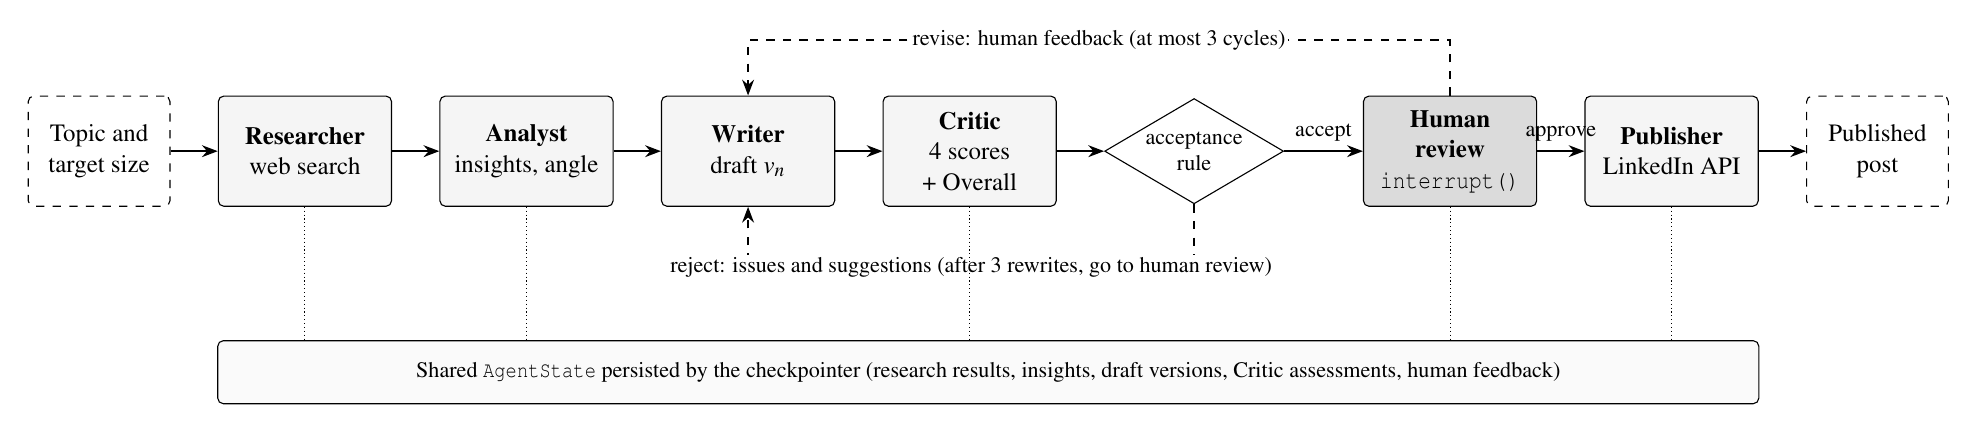
\begin{tikzpicture}[
  font=\small,
  node distance=6mm,
  agent/.style={draw, rounded corners=2pt, minimum width=22mm, minimum height=14mm, align=center, fill=gray!8},
  io/.style={draw, dashed, rounded corners=2pt, minimum width=18mm, minimum height=14mm, align=center},
  human/.style={agent, fill=gray!28},
  decision/.style={draw, diamond, aspect=1.7, align=center, inner sep=1pt, fill=white, font=\footnotesize},
  flow/.style={-{Stealth[length=2mm]}, thick},
  back/.style={-{Stealth[length=2mm]}, thick, dashed},
  lbl/.style={font=\footnotesize, fill=white, inner sep=1pt},
]
\node[io] (in) {Topic and\\target size};
\node[agent, right=of in] (res) {\textbf{Researcher}\\web search};
\node[agent, right=of res] (ana) {\textbf{Analyst}\\insights, angle};
\node[agent, right=of ana] (wri) {\textbf{Writer}\\draft $v_n$};
\node[agent, right=of wri] (cri) {\textbf{Critic}\\4 scores\\+ Overall};
\node[decision, right=of cri] (dec) {acceptance\\rule};
\node[human, right=10mm of dec] (hitl) {\textbf{Human}\\\textbf{review}\\\texttt{interrupt()}};
\node[agent, right=of hitl] (pub) {\textbf{Publisher}\\LinkedIn API};
\node[io, right=of pub] (out) {Published\\post};

\draw[flow] (in) -- (res);
\draw[flow] (res) -- (ana);
\draw[flow] (ana) -- (wri);
\draw[flow] (wri) -- (cri);
\draw[flow] (cri) -- (dec);
\draw[flow] (dec) -- node[above, font=\footnotesize] {accept} (hitl);
\draw[flow] (hitl) -- node[above, font=\footnotesize] {approve} (pub);
\draw[flow] (pub) -- (out);

\draw[back] (dec.south) -- ++(0,-8mm) -| node[lbl, pos=0.25] {reject: issues and suggestions (after 3 rewrites, go to human review)} (wri.south);
\draw[back] (hitl.north) -- ++(0,7mm) -| node[lbl, pos=0.25] {revise: human feedback (at most 3 cycles)} (wri.north);

\coordinate (sl) at ($(res.south west)+(0,-17mm)$);
\coordinate (sr) at ($(pub.south east)+(0,-25mm)$);
\draw[rounded corners=2pt, fill=gray!4] (sl) rectangle (sr);
\node[font=\footnotesize, align=center] at ($(sl)!0.5!(sr)$) {Shared \texttt{AgentState} persisted by the checkpointer (research results, insights, draft versions, Critic assessments, human feedback)};
\foreach \n in {res,ana,cri,hitl,pub} \draw[densely dotted] (\n.south) -- (\n.south |- sl);
\end{tikzpicture}}
\caption{Proposed pipeline. Solid arrows show the main execution flow and dashed arrows the two revision paths. The Critic's acceptance rule and the human checkpoint are the two validation stages.}
\label{fig:architecture}
\end{figure*}

\subsection{Critic Rubric}
\label{sec:rubric}

The Critic scores each post on four dimensions from 1 (\emph{very poor}) to 5 (\emph{excellent}), with a verbal anchor for every point of the scale (Appendix, Table~\ref{tab:rubric}):

\begin{itemize}
\item \textbf{Clarity and Readability}: whether the post is clear, understandable, well structured and easy to read, motivated by the role of message characteristics in the reactions to posts in professional groups \cite{rooderkerk2016nocomment};
\item \textbf{Relevance and Informational Value}: whether the post delivers substantive information for a professional audience and fulfils the intent of the requested topic \cite{usera2026linkedin};
\item \textbf{Professional Appropriateness}: whether tone, language and presentation suit a professional network and its audience \cite{usera2026linkedin};
\item \textbf{Engagement Quality}: whether the post attracts attention, sustains interest and invites appropriate professional interaction \cite{usera2025predicts}.
\end{itemize}

The dimensions come from prior studies of professional online communication; their combination into one anchored instrument shared by the Critic and human raters is part of the contribution.

The Critic receives the requested topic and the post, but not the Researcher's sources, so the rubric does not assess factual accuracy. Its output is a JSON object produced in a fixed order: a list of issues, each tagged with the dimension and the scale point it describes; the four dimension scores; and, last, a holistic \emph{Overall Quality} score from 1 to 5. The Overall score is elicited last so that it follows from the dimension-level assessment. It has no per-point anchors and is not used by the acceptance rule, which is why it does not equal the mean of the four dimensions. A coherence check in code flags any score higher than the worst anchor cited in the Critic's own issues for that dimension; the Critic is asked once to resolve the contradiction and, if it persists, the score is lowered to that anchor. The Critic does not rewrite the post.

\subsection{Acceptance Rule and Revision Loop}
\label{sec:rule}

The acceptance decision is computed in code from the scores rather than elicited from the model, so that the same rule can be applied to any set of scores. A post is accepted when the weighted composite $0.35\,\mathit{Cla} + 0.35\,\mathit{Rel} + 0.15\,\mathit{Pro} + 0.15\,\mathit{Eng}$ is at least 3.5 and no floor violation occurs; a floor violation means that two dimensions score below 3 and at least one of them is Clarity or Relevance. Clarity and Relevance weigh more because they determine whether the post informs at all. Checks that do not depend on judgment (length outside the target range, external links in the body, engagement bait) are applied as separate conformance checks, which also return the draft to the Writer but do not change the scores.

This rule replaced an earlier one under which a post was accepted when every dimension scored at least 3. On the development corpus, the earlier rule accepted all 22 runs at the first pass and never triggered a revision, since a score of 3 is anchored as \emph{acceptable}. The earlier rule had been fixed before data collection; the current rule was adopted on 8 September 2026, after the human data collection had started, and we report this as a deviation from the planned design. For the ten posts evaluated in Section~\ref{sec:evaluation}, both rules yield the same decision (accept).

When a post is rejected, the Critic's issues and suggestions are stored in the shared state and the workflow returns to the Writer. At most three automatic rewrites are allowed; after that, the post is forwarded to the human checkpoint with the Critic's assessment, which prevents repeated failures from producing an unbounded loop.

\subsection{Human-in-the-Loop Checkpoint}

Human intervention takes place after the Critic stage and before publication. The reviewer inspects the post together with the Critic's scores and either approves it, which forwards it to the Publisher, or returns it with free-text feedback, which routes it back to the Writer; the revised version passes through the Critic again before returning to the reviewer (Figure~\ref{fig:hitl}). At most three human revision cycles are allowed. While waiting for the reviewer, the execution is suspended with \texttt{interrupt()} and its state is persisted, so that the run resumes from the same point instead of restarting the pipeline. The Critic thus provides a repeatable assessment during generation, and the human reviewer provides contextual judgment before the irreversible publication step.

\begin{figure}[t]
\centering
\IfFileExists{figures/hitl-interface.png}{%
  \includegraphics[width=\columnwidth]{figures/hitl-interface.png}}{%
  \fbox{\parbox[c][3cm][c]{0.92\columnwidth}{\centering\TODO{export the upper panel of the original Figure 2 to figures/hitl-interface.png}}}}
\caption{Human review checkpoint in the user interface (example run). The reviewer sees the post, the Critic's scores (labelled \emph{Judge} in the interface) and the number of automatic rewrites and human revisions, and can publish the post, request a revision with free-text feedback, or cancel the run.}
\label{fig:hitl}
\end{figure}

\subsection{Implementation}

The system is implemented in TypeScript with LangGraph.js. The workflow is a \texttt{StateGraph} over a shared \texttt{AgentState}, and conditional edges implement the routing decisions associated with the acceptance rule and the human decision. Graph checkpoints are persisted by a file-backed extension of LangGraph's in-memory checkpointer, so interrupted runs survive server restarts. Every draft version and every Critic assessment is stored in a PostgreSQL database together with its provenance (Critic model, temperature, rubric version and a hash of the Critic prompt), so that scores produced by different Critic configurations cannot be mixed unnoticed. The user interface is a Next.js application whose API routes start and resume runs and stream progress to the browser through Server-Sent Events; execution traces can optionally be sent to LangSmith.

The Researcher and Analyst use OpenAI GPT-4o (\texttt{gpt-4o-2024-08-06}) at temperature 0.3, and the Writer uses a model of the GPT-4o family at temperature 0.9 (Section~\ref{sec:setup} reports which model wrote each evaluated post). The Critic uses GPT-4.1 (\texttt{gpt-4.1-2025-04-14}) at temperature 0.1; a model different from the Writer's was chosen to reduce self-preference bias \cite{panickssery2024llm}, although models of the same family may still share it. The Researcher queries the Tavily search API, and the Publisher uses the LinkedIn REST API. The full prompts of all agents (folder \texttt{prompts/}, generated from the running configuration, in the original Portuguese with an English translation in \texttt{prompts/en/}), the rubric and the analysis code are available at \TODO{anonymized repository URL}.
% ═════════════════════════════════════════════════════════════════════════════
\section{\uppercase{Evaluation}}
\label{sec:evaluation}

The evaluation addresses three research questions:

\begin{itemize}
\item[\textbf{RQ1}] To what extent do the Critic's scores agree with human ratings of the same posts, beyond the agreement expected by chance?
\item[\textbf{RQ2}] How reliable are the human ratings of these posts?
\item[\textbf{RQ3}] How stable are the Critic's scores across repeated runs, and do they respond to a clear degradation of the posts?
\end{itemize}

\subsection{Posts, Raters and Procedure}
\label{sec:setup}

\textbf{Posts.} The corpus consists of \NPosts{} LinkedIn posts in Brazilian Portuguese, generated by the pipeline between 29 August and 2 September 2026 for ten distinct topics on work and software development (Appendix, Table~\ref{tab:posts}). The posts have between \CharMin{} and \CharMax{} characters; three were requested with the small target size (500--900 characters) and seven with the medium size (1,200--1,800). All ten were accepted by the Critic at the first pass, with no automatic rewrite; none was submitted to the human checkpoint or published, so the evaluated versions are the first drafts. The Writer model was not constant: the agent configuration was changed during corpus generation, and the stored execution traces show that seven posts were written by GPT-4o (\texttt{gpt-4o-2024-08-06}) and three (J, L and P) by GPT-4o-mini (\texttt{gpt-4o-mini-2024-07-18}). The ten posts were taken from a development corpus of 16 accepted posts; \TODO{state how the ten posts were selected}.

\textbf{Raters.} \NRaters{} raters completed the questionnaire between 3 and 8 September 2026. \TODO{recruitment procedure, background (profession, LinkedIn use), native language and consent/ethics procedure}. The responses contain no identifying information.

\textbf{Questionnaire.} The questionnaire was implemented in Google Forms with one section per post, showing the requested topic followed by the post text; all raters saw the posts in the same order. For each post, raters answered five mandatory items on a five-point scale \cite{likert1932technique,krosnick1999maximizing}: the four rubric dimensions, worded with the same questions given to the Critic, followed by Overall Quality. \TODO{confirm whether the per-point anchors of Table~\ref{tab:rubric} were shown to the raters}. Raters were instructed to judge each dimension independently and not to assess factual accuracy, since neither they nor the Critic had access to the sources. The posts were not presented as AI-generated, and the Critic's scores were not disclosed. Each rater produced 50 ratings, for a total of 900.

\textbf{Critic scores.} The analyzed Critic scores are those stored for the same post versions, produced in one run per post with the final Critic configuration (GPT-4.1, temperature 0.1) on 8 September 2026; the post texts were not modified.\footnote{The previous version of this manuscript used a manually transcribed copy of the Critic scores in which post D was recorded as 4,3,4,3,3 instead of the stored 4,4,4,4,4. All results reported here are computed from the stored scores.} For RQ3, the Critic was run \RepRuns{} more times on each post with the same configuration, and once on a degraded version of each post truncated to its first 35\% of characters at a word boundary, for a total of \RepCalls{} calls; these runs did not replace the stored scores.

\subsection{Metrics}
\label{sec:metrics}

For each dimension, the Critic is compared with each rater on each post (\NCHperDim{} Critic--human comparisons per dimension), and every pair of raters is compared on each post (\NHHperDim{} human--human pairs per dimension). Exact agreement is the proportion of comparisons with identical scores, and within-one agreement the proportion that differ by at most one point. Values reported for the four dimensions are the mean over Clarity, Relevance, Professional Appropriateness and Engagement; Overall Quality is reported separately.

Percentage agreement does not discount the agreement produced by the score distributions alone, which is high when scores concentrate on few values. We therefore also report (a) the agreement expected by chance if both sources scored independently with their observed distributions, $\sum_k p_k q_k$ for exact agreement and analogously for within-one agreement, and (b) the agreement of a constant predictor that always outputs the most frequent human score. As chance-corrected and association measures we report the quadratic weighted kappa $\kappa_w$ \cite{cohen1968weighted} between Critic and human scores pooled over all comparisons, Spearman's $\rho$ between the Critic score and the mean human score of each post, and Krippendorff's ordinal $\alpha$ \cite{krippendorff2018content} among human raters. Score levels are compared through the mean difference (bias, Critic minus human) and the mean absolute error (MAE). To locate the source of human score variation, the sum of squares of each dimension is decomposed into rater and post components.

Since the independent units are posts and raters rather than individual comparisons, 95\% confidence intervals are obtained with a percentile bootstrap that resamples both posts and raters \cite{efron1994bootstrap}, with 2,000 replicates; pairs of a rater with its own resampled copy are discarded, and $\alpha$ is resampled over posts only. As a sensitivity analysis defined after inspecting the data, the analysis is repeated without the \FlaggedN{} raters who gave the minimum score to at least half of their ratings.

\subsection{Results}

\begin{table*}[t]
\centering
\caption{Exact and within-one ($\pm1$) agreement between pairs of human raters, between the Critic and human raters, and expected by chance for Critic--human comparisons given the observed score distributions. The confidence intervals come from the two-way bootstrap.}
\label{tab:agreement}
\small
% --- início de tables/agreement.tex (gerado) ---
\begin{tabular}{lcccccc}
\toprule
 & \multicolumn{2}{c}{Human--Human} & \multicolumn{2}{c}{Critic--Human} & \multicolumn{2}{c}{Chance (Critic--Human)} \\
\cmidrule(lr){2-3}\cmidrule(lr){4-5}\cmidrule(lr){6-7}
Dimension & Exact & $\pm1$ & Exact & $\pm1$ & Exact & $\pm1$ \\
\midrule
Clarity and Readability & 31.7\% & 71.0\% & 41.1\% & 89.4\% & 41.1\% & 89.4\% \\
Relevance and Informational Value & 26.9\% & 66.0\% & 21.7\% & 67.8\% & 20.4\% & 67.0\% \\
Professional Appropriateness & 30.1\% & 73.5\% & 42.2\% & 88.3\% & 41.8\% & 88.6\% \\
Engagement Quality & 25.2\% & 64.2\% & 22.2\% & 68.9\% & 24.1\% & 68.8\% \\
\midrule
\textbf{Four dimensions} & \textbf{28.4\%} & \textbf{68.7\%} & \textbf{31.8\%} & \textbf{78.6\%} & \textbf{31.9\%} & \textbf{78.4\%} \\
\quad 95\% CI & 21.0\%--36.5\% & 55.2\%--81.0\% & 22.8\%--40.8\% & 66.9\%--88.2\% & & \\
\midrule
Overall Quality & 27.1\% & 67.4\% & 23.3\% & 69.4\% & 24.0\% & 69.4\% \\
\bottomrule
\end{tabular}
% --- fim de tables/agreement.tex ---
\end{table*}

\begin{table*}[t]
\centering
\caption{Score levels and association. $M$ ($SD$): mean and standard deviation over all ratings; bias: Critic minus human; $\kappa_w$: quadratic weighted kappa between Critic and human scores; $\rho$: Spearman correlation between the Critic score and the mean human score per post ($n=10$; n/a when the Critic assigned the same score to all posts); $\alpha_H$: Krippendorff's ordinal alpha among human raters.}
\label{tab:scores}
\small
\begin{adjustbox}{max width=\textwidth}
% --- início de tables/scores.tex (gerado) ---
\begin{tabular}{lccccccc}
\toprule
Dimension & Human $M$ ($SD$) & Critic $M$ ($SD$) & Bias [95\% CI] & MAE & $\kappa_w$ & $\rho$ & $\alpha_H$ \\
\midrule
Clarity and Readability & 3.91 (1.11) & 4.00 (0.00) & +0.09 [$-$0.26, +0.48] & 0.76 & 0.00 & n/a & $-$0.02 \\
Relevance and Informational Value & 3.74 (1.19) & 3.20 (0.42) & $-$0.54 [$-$0.98, $-$0.05] & 1.12 & 0.01 & 0.13 & $-$0.01 \\
Professional Appropriateness & 3.93 (1.07) & 4.10 (0.32) & +0.17 [$-$0.22, +0.56] & 0.75 & 0.05 & 0.53 & $-$0.01 \\
Engagement Quality & 3.66 (1.23) & 3.30 (0.48) & $-$0.36 [$-$0.84, +0.13] & 1.11 & 0.00 & 0.04 & $-$0.02 \\
\midrule
Overall Quality & 3.77 (1.12) & 3.20 (0.42) & $-$0.57 [$-$1.01, $-$0.09] & 1.09 & $-$0.02 & $-$0.22 & $-$0.03 \\
\bottomrule
\end{tabular}
% --- fim de tables/scores.tex ---
\end{adjustbox}
\end{table*}

\subsubsection{Critic--Human Agreement (RQ1)}

Across the four dimensions, Critic--human exact agreement was \CHexAll{} (95\% CI \CHexLo{}--\CHexHi{}) and within-one agreement was \CHwAll{} (\CHwLo{}--\CHwHi{}), against \HHexAll{} and \HHwAll{} for pairs of human raters (Table~\ref{tab:agreement}). The agreement expected by chance from the score distributions, however, was \CHchanceExAll{} for exact and \CHchanceWAll{} for within-one agreement. The difference between observed and chance agreement lies between \ChanceDiffExLo{} and \ChanceDiffExHi{} percentage points for exact agreement and between \ChanceDiffWLo{} and \ChanceDiffWHi{} for within-one agreement (95\% CI). A constant predictor that always outputs the most frequent human score, which is 4 in every dimension, would reach \ConstExAll{} exact and \ConstWAll{} within-one agreement, more than the Critic.

The differences between dimensions follow from the same mechanism. Clarity and Professional Appropriateness show the highest Critic--human agreement (\CHexCla{} and \CHexPro{}) because the Critic almost always assigned 4, the most frequent human score, on these dimensions; Relevance and Engagement show the lowest (\CHexRel{} and \CHexEng{}) because the Critic mostly assigned 3. Consistently, $\kappa_w$ is close to zero in every dimension and the per-post correlation is weak or undefined (Table~\ref{tab:scores}); on Clarity the Critic assigned the same score to all ten posts, so no correlation can be computed.

\subsubsection{Reliability of Human Ratings (RQ2)}

The human raters did not agree with one another beyond chance either. Human--human exact agreement (\HHexAll{}) matches the chance expectation from the human score distribution (\HHchanceExAll{}; difference between \HHChanceDiffExLo{} and \HHChanceDiffExHi{} percentage points), and Krippendorff's ordinal $\alpha$ lies between \AlphaMin{} and \AlphaMax{} in all dimensions (Table~\ref{tab:scores}). The variance decomposition shows why: differences between posts account for only \VarPostMin{}--\VarPostMax{} of the variation in human scores, whereas differences between raters account for \VarRaterMin{}--\VarRaterMax{}, the remainder being rater-by-post variation. The mean human score of a post ranged only from \PostMeanMin{} to \PostMeanMax{} across the four dimensions. For these posts, a human score mainly reflects how lenient the rater is rather than which post was rated, which leaves little between-post signal for the Critic to agree with.

Score levels nevertheless differ between the two sources. The Critic's mean was close to the human mean on Clarity (bias \BiasCla{}) and Professional Appropriateness (\BiasPro{}), but lower on Relevance (\BiasRel{}, 95\% CI \BiasLoRel{} to \BiasHiRel{}) and Overall Quality (\BiasOve{}, \BiasLoOve{} to \BiasHiOve{}). The Critic's Engagement scores were also lower on average (\BiasEng{}), but the interval (\BiasLoEng{} to \BiasHiEng{}) includes zero. On Relevance and Overall Quality the Critic was therefore stricter than the average rater, which is not consistent with a uniformly permissive critic; its severity, however, was applied almost identically to every post.

\subsubsection{Critic Stability and Sensitivity (RQ3)}

\begin{table}[t]
\centering
\caption{Critic test--retest stability over \RepRuns{} repeated runs per post: mean within-post standard deviation, proportion of runs that reproduced the stored score, and proportion of posts whose runs were all identical.}
\label{tab:repeat}
\begin{adjustbox}{max width=\columnwidth}
% --- início de tables/repeat.tex (gerado) ---
\begin{tabular}{lccc}
\toprule
Dimension & Within-post $SD$ & Runs = reported score & Posts with identical runs \\
\midrule
Clarity and Readability & 0.00 & 100.0\% & 100.0\% \\
Relevance and Informational Value & 0.00 & 100.0\% & 100.0\% \\
Professional Appropriateness & 0.05 & 86.0\% & 90.0\% \\
Engagement Quality & 0.04 & 92.0\% & 90.0\% \\
Overall Quality & 0.10 & 94.0\% & 80.0\% \\
\bottomrule
\end{tabular}
% --- fim de tables/repeat.tex ---
\end{adjustbox}
\end{table}

The Critic's scores were stable (Table~\ref{tab:repeat}). The repeated runs reproduced the stored Clarity and Relevance scores in \RepEqualCla{} and \RepEqualRel{} of the cases. The remaining variation never exceeded one point and occurred on Professional Appropriateness (\RepEqualPro{} of the runs reproduced the stored score), Engagement (\RepEqualEng{}) and Overall Quality (\RepEqualOve{}). One stored score was not reproduced in any run (post L, Professional Appropriateness: 5 stored, 4 in all runs). The acceptance decision changed across runs for \RepFlips{} post (post H, whose Professional Appropriateness alternated between 4 and 3, moving its composite from 3.50 to 3.35).

The Critic did respond to a clear degradation. When posts were truncated to 35\% of their length, \TruncReject{} of them were rejected: the mean Engagement score fell from \RepMeanEng{} (repeated runs on the intact posts) to \TruncMeanEng{} and Clarity from \RepMeanCla{} to \TruncMeanCla{}. Relevance changed little (\RepMeanRel{} to \TruncMeanRel{}), and Professional Appropriateness was 4 for every truncated post. The low agreement in RQ1 is therefore not explained by random Critic noise: the Critic is consistent, and it distinguishes an intact post from a mutilated one, but it assigns nearly the same scores to all intact posts.

\subsubsection{Sensitivity Analysis}

Excluding the \FlaggedN{} raters who gave the minimum score to at least half of their ratings raised the mean human scores. This brought the human level closer to the Critic on Professional Appropriateness (bias \SensBiasPro{}) and moved it further away on Relevance (\SensBiasRel{}) and Overall Quality (\SensBiasOve{}), but did not change the conclusions: Critic--human exact agreement became \SensCHexAll{} against a chance expectation of \SensChanceExAll{}, human--human exact agreement became \SensHHexAll{}, and $\alpha$ remained close to zero (e.g., \SensAlphaCla{} for Clarity and \SensAlphaRel{} for Relevance).

% ═════════════════════════════════════════════════════════════════════════════
\section{\uppercase{Discussion}}
\label{sec:discussion}

A previous version of this study interpreted the similarity between Critic--human and human--human percentage agreement as evidence that the Critic remains close to human judgment. Once the agreement produced by the score distributions is taken into account, that interpretation does not hold: both percentages are what independent scoring with the same distributions would produce. Three observations explain this result and delimit what can be concluded.

First, the corpus has a restricted quality range. All posts were produced by the same pipeline and accepted by the Critic at the first pass, and the human raters did not distinguish between them. This is consistent with the Critic's own behavior: \CompAtThreshold{} of the ten posts obtained a composite of exactly 3.50, the acceptance threshold, and during development the same score vector (4, 3, 4, 3) was assigned to posts on unrelated topics. Under such conditions no rater, human or automated, can show agreement beyond chance, and percentage agreement mainly reflects how close the typical scores of the two sources are. Agreement studies of LLM critics embedded in generation pipelines therefore need items that span a meaningful quality range, for instance by adding degraded or human-written posts to the pipeline outputs, and should establish human reliability before interpreting critic--human agreement.

Second, the Critic behaves as a stable rater with coarse resolution and its own severity profile. It matches the average human level on Clarity and Professional Appropriateness, is stricter on Relevance and Overall Quality, rejects posts that lose most of their content, and, within the range of competent posts, does not rank them. Its Relevance scores in particular barely reacted to the removal of 65\% of each post. The Critic can therefore serve as a filter against clearly deficient drafts, but the present data provide no evidence that it discriminates among competent posts, which is precisely where the acceptance threshold operates. The decision flip observed for post H also shows that, with scores concentrated at the threshold, a one-point fluctuation is enough to change the outcome of the gate.

Third, for the architecture, these results argue against using the Critic's scores to rank posts or to justify skipping human review, and against calibrating the threshold on the Critic's own score distribution. Aligning the Critic's severity with the human level on Relevance would shift its scores without adding the missing discrimination. Whether the human checkpoint improves the published content was not examined in this study; the results only indicate that the Critic cannot replace it for posts in this quality range.

\subsection{Limitations}
\label{sec:limitations}

The evaluation uses ten posts in a narrow quality range, all accepted at the first pass; no post rejected by the Critic was available, so the results say nothing about the Critic's behavior on the rejected side of the threshold, beyond the truncation control. The architecture itself was not evaluated: there is no comparison with single-prompt generation or with the pipeline without the Critic, no measurement of revision counts, human rejection rates, latency or cost, and the human checkpoint was not exercised in the study. The results concern a single Critic configuration (GPT-4.1 with one prompt at temperature 0.1), one language (Brazilian Portuguese) and one platform; an earlier version of the Critic prompt had scored the same texts differently in at least one dimension for five of the ten posts. The Writer model was not held constant across the corpus (GPT-4o for seven posts, GPT-4o-mini for three). The raters are a convenience sample \TODO{describe}, and the conclusions concern these raters rather than a population. All raters saw the posts in the same order, so fatigue is confounded with post identity. The acceptance rule was changed after data collection had started, and the rater exclusion criterion of the sensitivity analysis was defined after inspecting the data.

% ═════════════════════════════════════════════════════════════════════════════
\section{\uppercase{Conclusion}}
\label{sec:conclusion}

This paper presented a Human-in-the-Loop multi-agent architecture for professional social media content generation, in which Researcher, Analyst, Writer, Critic and Publisher agents are coordinated through a stateful graph, an LLM Critic drives a bounded revision loop through an acceptance rule computed from an anchored rubric, and a human checkpoint precedes publication.

We compared the Critic with \NRaters{} human raters on \NPosts{} posts produced and accepted by the pipeline. Raw agreement was similar for Critic--human and human--human comparisons, but neither exceeded the agreement expected by chance, and human ratings had no measurable reliability: differences between raters, not between posts, explained the human score variation. The Critic was stable across repeated runs, rejected most posts truncated to about a third of their length, and was stricter than humans on Relevance and Overall Quality, but it assigned almost the same scores to all intact posts.

The main lesson is methodological. Evaluating an LLM critic on the outputs of the pipeline it controls restricts the quality range to the point where agreement statistics lose their meaning, and percentage agreement without a chance baseline can then suggest an alignment that is not there. Future work will evaluate the Critic on corpora that span the quality range, including degraded and human-written posts; compare the architecture with single-prompt generation and with a pipeline without the Critic, using operational measures such as revisions, human rejection rate, latency and cost; include several Critic models; and use larger rater panels with randomized post order.

\section*{\uppercase{Acknowledgements}}

The authors acknowledge the use of an AI assistant to review the manuscript for grammar and style and to support the data analysis scripts. The authors are responsible for all the content, interpretations and conclusions presented in this paper.

\bibliographystyle{apalike}
{\small
\bibliography{refs}}

% ═════════════════════════════════════════════════════════════════════════════
\section*{\uppercase{Appendix}}

\begin{table*}[h]
\centering
\caption{Rubric used by the Critic and the human questionnaire (translated from Brazilian Portuguese). Scale labels: 1 very poor, 2 poor, 3 acceptable, 4 good, 5 excellent. Overall Quality (``All things considered, what is the overall quality of this post?'') has no per-point anchors.}
\label{tab:rubric}
\scriptsize
\setlength{\tabcolsep}{3pt}
\renewcommand{\arraystretch}{1.15}
\begin{tabularx}{\textwidth}{@{}>{\raggedright\arraybackslash}p{2.5cm}*{5}{>{\raggedright\arraybackslash}X}@{}}
\toprule
Dimension and question & 1 & 2 & 3 & 4 & 5 \\
\midrule
\textbf{Clarity and Readability.} Is the post clear, understandable, well structured and easy to read? &
Confusing. Dense block or overly long sentences; the central idea cannot be identified. &
Hard to follow. Weak structure, requires re-reading; the idea only appears at the end, or not at all. &
Understandable with average effort. Acceptable structure, but some passages are dense, truncated or repetitive. &
Clear and well organized. Fluent reading, central idea evident early, line breaks help. &
Exceptionally clear. Each paragraph advances the idea; rhythm and formatting serve the reader; nothing is superfluous. \\
\midrule
\textbf{Relevance and Informational Value.} Does the post deliver meaningful, substantive information appropriate for a professional audience and fulfil the intent of the topic? &
No value or off-topic. Informs nothing and/or does not address the intent of the topic. &
Generic. Common sense and broad claims without substance; only grazes the topic. &
Correct but predictable information. Covers the basics of the topic without adding much for people in the field. &
Substantive. Provides a data point, example or useful distinction and addresses the intent of the topic well. &
High value. Non-obvious, specific and actionable insight for the professional audience. \\
\midrule
\textbf{Professional Appropriateness.} Are the tone, language and presentation appropriate for a professional social network and the intended audience? &
Inappropriate. Offensive, sensationalist, jarringly informal or aggressively promotional. &
Out of place. Exaggeration, clickbait, empty marketing jargon, excessive emojis or punctuation. &
Acceptable. Nothing improper, but the register fluctuates or sounds impersonal and generic (``AI text''). &
Appropriate. Consistent and authentic professional tone; language suited to the audience. &
Exemplary. Credible and natural professional voice, calibrated to the audience, free of clichés. \\
\midrule
\textbf{Engagement Quality.} Does the post attract attention, sustain interest and encourage appropriate professional interaction? &
Does not hold attention. Opening without a hook and nothing to sustain reading, or an artificial request for interaction. &
Weak. Slow start and interest drops midway; generic invitation such as ``what do you think?''. &
Average. Functional opening, keeps the reader until the end; invitation present but not very specific. &
Good. Scroll-stopping opening, sustained interest, invitation anchored in the content of the post. &
Excellent. The first line compels reading on, tension is maintained, and the invitation draws on a specific experience of the reader. \\
\bottomrule
\end{tabularx}
\end{table*}

\begin{table*}[h]
\centering
\caption{Evaluated posts in questionnaire order: requested topic (translated), length in characters, stored Critic scores (Clarity, Relevance, Professional Appropriateness, Engagement, Overall) and mean human score per dimension.}
\label{tab:posts}
\footnotesize
% --- início de tables/posts.tex (gerado) ---
\begin{tabular}{lp{6.2cm}rlccccc}
\toprule
 & & & & \multicolumn{5}{c}{Human mean} \\
\cmidrule(lr){5-9}
Post & Requested topic (translated) & Chars & Critic & Cl. & Rel. & Prof. & Eng. & Ov. \\
\midrule
A & What is technical debt and how can it be explained to non-technical people? & 896 & 4,3,4,4,3 & 4.2 & 3.9 & 4.0 & 3.7 & 4.0 \\
J & Junior programmers will no longer be hired from 2027 onwards & 1361 & 4,3,4,3,3 & 4.2 & 4.2 & 4.2 & 4.1 & 4.1 \\
D & Legacy code that nobody wants to touch and nobody manages to replace & 1867 & 4,4,4,4,4 & 3.9 & 3.8 & 4.1 & 3.7 & 3.7 \\
L & Why do retrospective meetings change nothing? & 1686 & 4,3,5,3,3 & 3.9 & 3.8 & 4.2 & 3.7 & 3.7 \\
F & Technical certifications have lost value in hiring processes & 1227 & 4,3,4,3,3 & 3.7 & 3.6 & 3.8 & 3.7 & 3.8 \\
P & A college degree is no longer of any use in the job market & 1197 & 4,4,4,4,4 & 3.8 & 3.8 & 3.7 & 3.6 & 3.7 \\
I & Artificial intelligence will transform the future of work & 1309 & 4,3,4,3,3 & 3.6 & 3.9 & 3.6 & 3.7 & 3.8 \\
E & How to double a development team's productivity in 30 days? & 938 & 4,3,4,3,3 & 3.8 & 3.4 & 3.8 & 3.3 & 3.6 \\
H & What is the future of programming? & 1555 & 4,3,4,3,3 & 3.7 & 3.4 & 3.7 & 3.4 & 3.5 \\
C & Daily stand-up meetings have become an empty ritual in most tech teams & 1183 & 4,3,4,3,3 & 4.2 & 3.7 & 4.1 & 3.7 & 3.8 \\
\bottomrule
\end{tabular}
% --- fim de tables/posts.tex ---
\end{table*}

\begin{table}[h]
\centering
\caption{Score distribution (\% of ratings, human / Critic) per dimension.}
\label{tab:distribution}
\begin{adjustbox}{max width=\columnwidth}
% --- início de tables/distribution.tex (gerado) ---
\begin{tabular}{lccccc}
\toprule
Dimension & 1 & 2 & 3 & 4 & 5 \\
\midrule
Clarity and Readability & 7 / 0 & 4 / 0 & 15 / 0 & 41 / 100 & 33 / 0 \\
Relevance and Informational Value & 7 / 0 & 9 / 0 & 16 / 80 & 38 / 20 & 30 / 0 \\
Professional Appropriateness & 6 / 0 & 4 / 0 & 14 / 0 & 43 / 90 & 33 / 10 \\
Engagement Quality & 9 / 0 & 8 / 0 & 19 / 70 & 35 / 30 & 28 / 0 \\
Overall Quality & 6 / 0 & 7 / 0 & 21 / 80 & 38 / 20 & 29 / 0 \\
\bottomrule
\end{tabular}
% --- fim de tables/distribution.tex ---
\end{adjustbox}
\end{table}

\end{document}
